% Template for ICASSP-2020 paper; to be used with:
%          spconf.sty  - ICASSP/ICIP LaTeX style file, and
%          IEEEbib.bst - IEEE bibliography style file.
% --------------------------------------------------------------------------
\documentclass{article}
\usepackage{spconf,amsmath,graphicx,xcolor,hyperref}
\hypersetup{
    colorlinks=true,
    linkcolor=blue,
    filecolor=magenta,
    urlcolor=blue,
    bookmarks=true,
    citecolor=magenta,
}
% Example definitions.
% --------------------
\def\x{{\mathbf x}}
\def\L{{\cal L}}

\newcommand{\ml}[1]{\textcolor{blue}{ML : #1}}
\newcommand{\fg}[1]{\textcolor{red}{FG : #1}}

% Title.
% ------
\title{Bandwidth extension of musical audio signals with no side information using dilated convolutional neural networks}
%
% Single address.
% ---------------
\name{Mathieu Lagrange, F\'elix Gontier \thanks{Work partially funded by ANR CENSE}}
\address{LS2N, CNRS, Centrale Nantes}
%
% For example:
% ------------
%\address{School\\
%	Department\\
%	Address}
%
% Two addresses (uncomment and modify for two-address case).
% ----------------------------------------------------------
%\twoauthors
%  {A. Author-one, B. Author-two\sthanks{Thanks to XYZ agency for funding.}}
%	{School A-B\\
%	Department A-B\\
%	Address A-B}
%  {C. Author-three, D. Author-four\sthanks{The fourth author performed the work
%	while at ...}}
%	{School C-D\\
%	Department C-D\\
%	Address C-D}
%

\renewcommand{\baselinestretch}{.98}

\begin{document}
%\ninept
%
\maketitle
%
\begin{abstract}

Bandwidth extension has a long history in audio processing. While speech processing tools do not rely on side information, production-ready bandwidth extension tools of general audio signals rely on side information that has to be transmitted alongside the bitstream of the low frequency part, mostly because polyphonic music has a more complex and less predictable spectral structure than speech.

This paper studies the benefit of considering a dilated fully convolutional neural network to perform the bandwidth extension of musical audio signals with no side information on the magnitude spectra. Experimental evaluation using two public datasets, \textit{medley-solos-db} and \textit{gtzan}, respectively of monophonic and polyphonic music demonstrate that the proposed architecture achieves state of the art performance.

\end{abstract}
%
\begin{keywords}
Artificial audio bandwidth extension, deep neural network, musical audio processing
\end{keywords}
%
\section{Introduction}
\label{sec:intro}

Bandwidth extension has a long standing history in telecommunication where the bitrate allowed by the given application may be reduced \cite{larsen2005audio}. In that case, it is often beneficial to preserve a good perceptual quality in the lower frequencies, for example to preserve intelligibility in speech applications. It is thus useful to consider a processing unit on the receiver that is able to produce a wide-band signal in order to improve perceived quality given the narrow band signal consisting of the lower frequencies, typically up to 4 kHz for speech.

Many techniques have been introduced for speech, and most of them operate on the magnitude spectra, where the spectral envelope of the narrow band signal is used to predict the spectral envelope of the higher frequencies. Recent approaches consider deep neural networks to do so \cite{abel2017artificial}. This approach assumes a source-filter model for speech production and requires some integration of two processing units, one responsible for the narrow band signal decoding and one responsible for the bandwidth extension. Extension on the magnitude spectra using a deep neural architecture has been proposed in \cite{li2015deep}. Recurrent neural networks \cite{ling2018waveform} or Wavenet architectures can also be considered \cite{gupta2019speech}. In this case, the network directly predicts the wide band speech signal, given some information provided by the conditioning stack that processes the narrow band signal. This approach is very flexible, but still computationally demanding.

Due to interoperability requirements in telephony, the bandwidth extension process in speech is done without any side information. That is, the processing unit on the decoder side has to predict the higher frequency signal given some static knowledge and the lower frequency signal only.

In general audio coding, bandwidth extension has been introduced in the beginning of the millennium \cite{dietz2002spectral}. General audio coding is more complex than speech coding due to the variety of physical sources that may produce the signal that has to be encoded. Due to this, and the ability to control the whole transmission stack for most use cases, some side information is considered to perform the bandwidth extension process. This side information is computed using the wide band signal at the encoder side and transmitted within the bitstream. In \cite{dietz2002spectral}, the main concept introduced is called spectral band replication (SBR) where the lower frequencies of the magnitude spectra are duplicated and transposed. Due to the typical exponential decay of magnitude with respect to the frequency, the overall magnitude of the transposed spectra has to be adjusted.

Some post processing steps can be undertaken to further improve the perceptual quality. As the encoder has access to the SBR prediction and the reference high frequency spectra, it is able to adapt to some special cases where considering the high frequency spectrum as the low frequency one will fail. For example, some high frequency tones that are perceptually salient may not be be recreated using the replication process. In this case, an additional processing unit can be considered to produce salient sinusoidal components \cite{ekstrand2002bandwidth}. The lower frequencies may have strong harmonics and the higher ones only noise like components. In this case, an inverse filtering is applied \cite{ehret2004audio}. Extension for low delay applications have been proposed \cite{friedrich2007spectral}, as well as the application of the phase vocoder \cite{flanagan1966phase} to reduce unpleasant roughness typically introduced when considering SBR tools \cite{nagel2009harmonic}.

Learning approaches, such as non-negative matrix factorization \cite{sun2013non}, and deep learning approaches \cite{miron2018high} have several benefits compared to algorithmic approaches discussed above. First, there may be no need for side information if the capacity of the model is sufficient to encode the rich relationship between the lower frequencies and the higher frequencies of the spectrum and if those encoded relationships are generic enough to produce satisfying results for real use case scenarios. Secondly, the relationships encoded by the model being non explicit, there is less chance of reaching a "glass-ceiling" in terms of perceptual quality.

To investigate further in this direction, we consider in this paper a deep convolutional network that operates in the magnitude spectrum. The model is described in Section \ref{sec:model}. Its performance is evaluated using an experimental protocol described in Section \ref{sec:protocol} on two public datasets: the \textit{medley-solos-db} and the \textit{gtzan} datasets\footnote{The code is available at \url{https://github.com/mathieulagrange/paperBandwidthExtensionCnn} and some audio examples can be listened to at \url{https://mathieulagrange.github.io/paperBandwidthExtensionCnn/demo}.}. Outcomes of the performance analysis are described in Section \ref{sec:experiments} and discussed in Section \ref{sec:discussion}.

Our main findings are that: 1) use of dilated convolutional filters lead to architectures that are less sensitive to the tuning of the other meta-parameter and reduce the complexity of the model while preserving a receptive field adapted to the task at hand, 2) compressive architectures like autoencoders do not perform favorably compared to a fully convolutional neural network without compression.

\section{Model}
\label{sec:model}

The aim of a bandwidth extension system is to predict the high frequency part of the spectrum. In this paper, we consider audio data represented as magnitude spectra. The input and the output of the model consist in 128x10 (frequency x time) matrices that respectively represent the low frequency and high frequency parts of the audio for an approximate duration of $160$ms (more details are provided in Section \ref{sec:protocol}).

The architecture is a fully convolutional neural network \cite{long2015fully} with $L$ layers followed by rectified linear units (ReLU) activations, as described in Figure~\ref{fig:mdl}. The number of output convolution channels $C$ is the same for all hidden layers. Convolution kernels also share the same size $(K_t, K_f)$ in the time and frequency dimensions respectively. To keep the shape of magnitude spectra constant throughout the network, representations at the input of each layer are padded by replicating their boundary values depending on the kernel size. Dilated convolutions are considered to artificially increase the receptive field of the model \cite{yu2016multi}, allowing it to capture patterns on larger scales without added parameters. From a signal processing standpoint, this procedure is equivalent to applying the convolution on a down-sampled version of the input. A fixed dilation ratio $D$ is used in the frequency dimension for hidden layers, and no dilation is used in the input and output layers of the network. As a result each hidden layer increases the receptive field by $D(K-1)$ frequency bins compared to $K-1$ without dilation.

\begin{figure}[t]
    \centering
    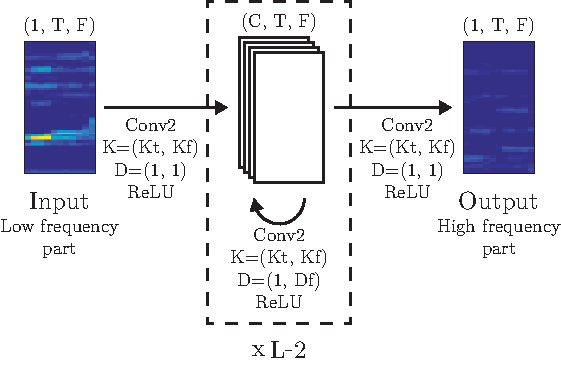
\includegraphics[width=\columnwidth]{figures/mdl.pdf}
    \caption{Proposed deep convolutional neural network architecture for bandwidth extension.}\label{fig:mdl}
    \vspace{-2mm}
\end{figure}

The model is trained using the mean squared error (MSE) loss function. Optimization is performed using the Adam \cite{kingma2014adam} algorithm with minibatches of $64$ examples and a learning rate of $0.001$.

% of expression:
% \begin{equation}
% L(y, \hat y) = \frac{1}{N_b}\sum\limits_{n=1}^{N_b}\sum\limits_{t=1, f=1}^{T, F}(\hat y_n(t, f) - y_n(t, f))^2
% \end{equation}
% where $y_n(t, f)$ is the ground truth high frequency part of the spectrum, $\hat y_n(t, f)$ is the output of the model, $N_b$ is the batch size, ant $T$ and $F$ are the time and frequency dimensions of the output respectively.

Reverting to the time domain requires the estimation of the phase information for higher frequencies whose magnitude have been predicted. Several methods proposed in the literature are considered. For evaluation purposes, the phase can be the original phase, termed \textit{oracle} in the following, the low frequency phase as proposed in \cite{miron2018high} and a flipped version of the low frequency phase as proposed in \cite{li2015deep}, termed \textit{mirror} in the following. The latter gave consistently better results, so only the results achieved using this method are reported.

\section{Experimental protocol}
\label{sec:protocol}

\subsection{Datasets}

Two datasets are considered in this study to evaluate the performance of the proposed model, the \textit{medley-solos-db} dataset \cite{lostanlen2016deep}, and the \textit{gtzan} dataset \cite{tzanetakis2002musical}. The first has 21572 monophonic audio clips of about 3 seconds, for a total duration of about 18 hours. The second comprises 100 polyphonic pop songs of 30 seconds each for each of the 10 musical genres represented, for a total duration of about 8 hours. The \textit{medley-solos-db} dataset is already split into "training", and "test" datasets, they are considered as is in this study. The \textit{gtzan} dataset is split in a train set and a test set using the following procedure. For each genre, the first 70 songs are put in the train set and the remaining 30 in the test set.

For both datasets, the audio data is resampled to $8$kHz and converted to spectral data using a short-term Fourier transform (STFT) with frame size of $256$ samples, hop size of $128$ samples and a Hann window. Extracts are further split into "textures" of $10$ frames, processed as individual examples.

The resulting spectra are split into 2 parts, the low frequency one, that serves as input to the different models and the high frequency one that serves as reference for training the models and computing the evaluation metrics.

\subsection{Metrics}


Three metrics are considered. The first metric is the average loss on the test set used to get a global understanding of the behavior of the predictors in the spectral domain. The second metric is the average signal-to-reconstruction ratio (SRR), computed in the time domain. Complex spectral values are computed for each batch of textures using the original phase for the low frequency part and one of several estimates for the high frequency part. The time domain signal is obtained by performing an inverse STFT on the complex spectra with the \textit{oracle} phase and the \textit{mirror} phase.

As it will be discussed in Section \ref{sec:experiments}, loss of phase correspondence between the predicted and reference complex spectra lead to the SRR being no longer relevant as a performance metric. Ultimately, subjective evaluation by means of listening tests performed by humans is desirable. However, setting up those tests is time consuming and considering the whole datasets as stimuli is impractical. This issue is left for future research.

A good alternative is the use of objective metrics based on perceptual models that have been proposed and used with success in many audio signal processing tasks, such as the PEASS, a perceptual evaluation method for the evaluation of audio source separation tools \cite{emiya2011subjective}. While some metrics provided are specific to the  audio source separation task, the overall perceptual score (OPS) is suitable for providing an estimate of the perceptual impact of a degraded signal over a reference one.

% overall difference grade (odg) of the perceptual evaluation of audio quality tool (peaq) \cite{thiede2000peaq} and

\subsection{Baselines}

Three baselines are considered. The first is a simplified version of the SBR technique, where the high frequency part is simply the low frequency part whose amplitudes are scaled. This baseline requires some side information, that is the amplitude scaling factor defined as the ratio of average amplitude between the high frequency part and the low frequency one, computed for each texture.

The second and the third ones are reimplementations of the deep architectures presented in \cite{miron2018high}. The \textit{cnn bottleneck} encoder part consists in two convolutional layers with filters of size $(1, F)$ and $(T, 1)$ that independently summarize information in the frequency and time dimensions of the input data respectively. A fully connected layer is then applied to extract a code of $64$. The decoder part mirrors these processing steps to recover a spectrum with the original input size. This model is implemented as described in \cite{miron2018high}, though with different filter sizes as $F=128$ and $T=10$ to match the data format considered in this study. The \textit{cnn stride2} autoencoder adopts a different strategy where frequency patterns information is extracted at multiple scales using strided convolutions. The first four layers operate independently on each time frame, and are followed by two convolutional layers with square kernels. The number of channels increases linearly with each additional layer. In this study, the first two layers are removed to account for the difference in the size of the frequency dimension in considered spectra. %For both architectures input examples are logarithmically scaled using the function $log_{10}(1+x)$ to account for the magnitude difference between low and high frequencies, as described by the authors.

%\footnote{Note for reviewers, some other preprocessing steps taken in \cite{miron2018high}, like logarithmical scaling and normalization are not implemented as they lead to numerical instabilities which are still under study. We also contacted the authors that will send us the train/test split. This will hopefully allow us to add the medleys dataset to the study.}

Additionally, two anchors are considered: the \textit{oracle} predictor that "predicts" the actual high frequency spectral pattern and the \textit{null} predictor that outputs a vector of zeros.

\section{Experiments}
\label{sec:experiments}

The experiments reported here are conducted in order to study two main design issues for the task at hand: 1) the impact of the dilation on the other meta parameters, and 2) the impact of the compression used in the design of autoencoders.

\begin{figure*}[t]
\center
\begin{tabular}{cc}
  (a) & (b) \\
  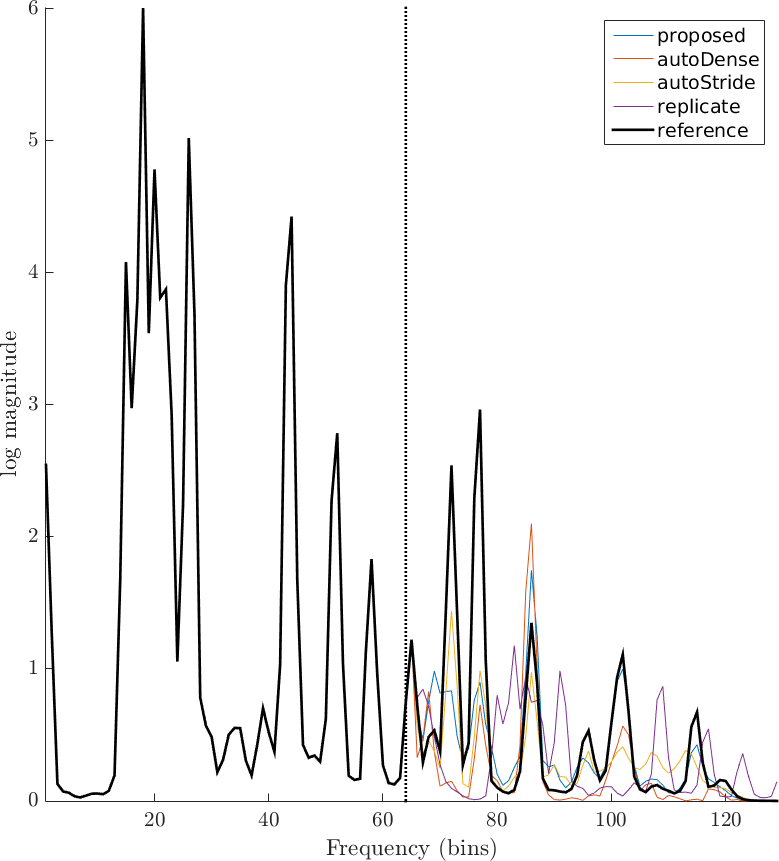
\includegraphics[width = .9\columnwidth]{figures/solos_1141.png}
&
  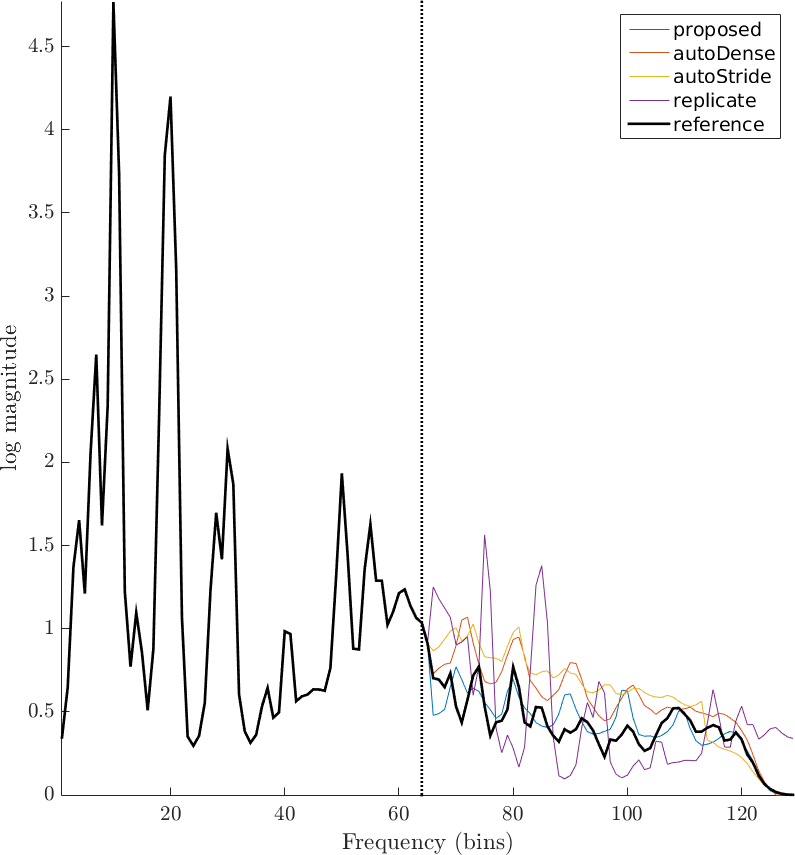
\includegraphics[width = .9\columnwidth]{figures/gtzan_1120.png}
\end{tabular}
\caption{Examples of predictions for (a) the \textit{medley-solos-db} dataset and (b) the \textit{gtzan} dataset. The proposed model handles correctly the harmonic structures (a) and the average magnitude of more complex spectral shapes (b).}
\label{fig:spec}
\vspace{-2mm}
\end{figure*}

%\subsection*{Dilation}

The dilation parameter $D$ is a very interesting feature of convolutional networks as it allows us to expand the receptive field without increasing the model complexity. The other parameters that control its size are $K$ the size of the filters, and $L$ the number of layers. As can be seen on Table \ref{tab:kvsd}, $D=2$ allows us to reduce the loss and also to reduce the gain achieved by increasing $K$. The effect is more important on the \textit{gtzan} dataset. Table \ref{tab:lvsd} shows the same effect of $D$ on $L$. %As predictable, this regularization effect is not present on $C$ (not shown due to space constraints). %see Table \ref{tab:cvsd}.
%\fg{Enlever la derniere phrase ou l'expliciter}

Increasing further the dilation factor to $D=3$ is not beneficial, as the receptive field is sufficiently large with $D=2$. Indeed, with $D=2$, $K=17$, $L=6$, it lead to a receptive field size of $89$ where the input and output of the predictor is of size $64$. This setting with $C=64$ is selected for the remaining of the experiments.

%
% \fg{formule pour calculer la taille du receptive field, same en temps: input layer + Hidden layers + Output layer}
% \begin{equation}
% R_f = K_f + (L-2)D\frac{K_f-1}{2} + \frac{K_f-1}{2}
% \end{equation}


\begin{table}[t]
  \caption{Spectral loss on the testing set for the proposed architecture with $L=7$ and $C=64$.}
  \label{tab:kvsd}
  \begin{center}
\begin{tabular}{llcc}
$K$ & dilation ($D$) & \textit{gtzan} & \textit{medley-solos-db} \\
\hline
13 & 1 & 0.109 $\pm$0.020 & 0.237 $\pm$0.014 \\
17 & 1 & 0.105 $\pm$0.021 & 0.226 $\pm$0.016 \\
13 & 2 & 0.102 $\pm$0.021 & 0.226 $\pm$0.017 \\
17 & 2 & 0.102 $\pm$0.022 & 0.218 $\pm$0.019 \\
% 13 & 3 & - $\pm$- &     - $\pm$- \\
% 17 & 3 & 0.103 $\pm$0.022 &     - $\pm$- \\
\end{tabular}
  \end{center}
  \vspace{-4mm}
\end{table}

\begin{table}[t]
  \caption{Spectral loss on the testing set for the proposed architecture with $K=17$ and $C=64$.}
  \label{tab:lvsd}
  \begin{center}
\begin{tabular}{llcc}
$L$ & dilation ($D$) & \textit{gtzan} & \textit{medley-solos-db} \\
\hline
5 & 1 & 0.110 $\pm$0.017 & 0.240 $\pm$0.013 \\
6 & 1 & 0.107 $\pm$0.021 & 0.231 $\pm$0.016 \\
7 & 1 & 0.105 $\pm$0.021 & 0.226 $\pm$0.016 \\
5 & 2 & 0.102 $\pm$0.019 & 0.228 $\pm$0.015 \\
6 & 2 & 0.102 $\pm$0.022 & 0.225 $\pm$0.019 \\
7 & 2 & 0.102 $\pm$0.022 & 0.218 $\pm$0.019 \\
% 5 & 3 & - $\pm$- &     - $\pm$- \\
% 6 & 3 & - $\pm$- &     - $\pm$- \\
% 7 & 3 & 0.103 $\pm$0.022 &     - $\pm$- \\
\end{tabular}
\end{center}
\vspace{-4mm}
\end{table}





% \begin{table}[t]
% \begin{tabular}{llcc}
% $C$ & dilation ($D$) & gtzan & medleysolos \\
% \hline
%  32 & 1 & 0.108 $\pm$0.020 & 0.237 $\pm$0.014 \\
%  64 & 1 & 0.107 $\pm$0.021 & 0.231 $\pm$0.016 \\
% 128 & 1 & 0.107 $\pm$0.019 & 0.233 $\pm$0.014 \\
%  32 & 2 & 0.102 $\pm$0.021 & 0.229 $\pm$0.016 \\
%  64 & 2 & 0.102 $\pm$0.022 & 0.225 $\pm$0.019 \\
% 128 & 2 & 0.101 $\pm$0.020 & 0.220 $\pm$0.017 \\
% \end{tabular}
% \caption{Loss on the testing set for the proposed architecture with $K=17$ and $L=7$.}
% \label{tab:cvsd}
% \end{table}

%\subsection*{Full cnn versus autoencoders}

Compared to the two encoder-decoder baselines, the proposed approach compares favorably in terms of spectral loss, see Table \ref{tab:loss}. An advantage of considering spectral bandwidth extension as task is the ease of fine grain performance analysis. Contrary to classification pipelines, the input and the output of the network are equivalent in terms of physical interpretation. It allows us to visually interpret the behavior of the predictors. As can be seen on Figure \ref{fig:spec}, the proposed model handles correctly the harmonic structures and the average magnitude of more complex spectral shapes.

\begin{table}[t]
  \caption{Spectral loss over the test set.}
  \label{tab:loss}
  \begin{center}
\begin{tabular}{lcc}
method & \textit{gtzan} & \textit{medley-solos-db} \\
\hline
proposed & 0.102 $\pm$0.022 & 0.225 $\pm$0.019 \\
cnn bottleneck & 0.107 $\pm$0.017 & 0.241 $\pm$0.011 \\
cnn stride2 & 0.110 $\pm$0.017 & 0.228 $\pm$0.013 \\
\end{tabular}
\end{center}
\vspace{-4mm}
\end{table}

In order to evaluate the proposed approach in the time domain, the SRR is considered. As can be seen on Table \ref{tab:SRR}, there is a direct inverse correlation between the spectral loss and the SRR when considering the oracle phase. Considering the mirror phase strongly reduces the phase correlation between the reference and the estimate leading to low SRR even for the oracle magnitude estimator. Though, informal listening test shows that considering the oracle estimator using the mirror phase estimate is perceptually more pleasing than the null predictor. We conclude that the sensitivity of the SRR to phase shift reduces its usefulness and turn to an objective perceptual measure to better assess the performance of the predictors.

As can be seen on Table \ref{tab:OPS}, the proposed approach improves over the baselines in terms of OPS (the higher the better). Whereas the autoencoder architectures appears to perform similarly in terms of SRR, they have different behavior when considering the OPS metric, the stride being more effective on monophonic music and the dense being more adapted to polyphonic music.

% \ml{perform ttest when all computation is done}

\begin{table}
  \caption{SRR achieved by the different methods on the \textit{medley-solosdb} and the \textit{gtzan} datasets using the \textit{mirror} and \textit{oracle} phase estimates.}
  \label{tab:SRR}
  \begin{center}
\begin{tabular}{lcc|cc}
  & \multicolumn{2}{c|}{\textit{medley-solos-db}} & \multicolumn{2}{c}{\textit{gtzan}} \\
  method & mirror & oracle & mirror & oracle \\
\hline
null & 12.9 $\pm$3 & 12.9 $\pm$3 & 12.9 $\pm$3 &  12.9 $\pm$3\\
replicate & 10.7 $\pm$3 & 11.6 $\pm$3 & 10.8 $\pm$3 & 13.3 $\pm$3\\
\hline
cnn bottleneck & 10.6 $\pm$2 &  13.3 $\pm$3 & 11.1 $\pm$3 & 15.6 $\pm$3 \\
cnn stride2 & 11.2 $\pm$3 & 13.9 $\pm$3 & 11.2 $\pm$3 & 15.6 $\pm$3 \\
\hline
proposed  & 11.0 $\pm$2 & 14.3 $\pm$3  & 11.3 $\pm$3 & 16.3 $\pm$3 \\
\hline
oracle & 10.5 $\pm$3 & $\infty$ & 10.5 $\pm$3 & $\infty$ \\
\end{tabular}
\end{center}
\vspace{-4mm}
\end{table}

% \begin{table}[t]
%   \begin{tabular}{lcc}
%   method   & mirror & oracle \\
%   \hline
%   null & 12.91 $\pm$3.26 &  12.91 $\pm$3.26 \\
%   replicate & 10.84 $\pm$3.30 & 13.30 $\pm$3.22 \\
% \hline
%   cnn bottleneck & 11.14 $\pm$2.98 & 15.62 $\pm$3.23 \\
%   cnn stride2 & 11.20 $\pm$2.84 & 15.58 $\pm$3.10 \\
%   \hline
%   proposed  & 11.28 $\pm$2.98 & 16.32 $\pm$3.31\\
%   \hline
%   oracle & 10.51 $\pm$3.26 & $\infty$ \\
%   \end{tabular}
%   \caption{SRR achieved by the different methods on the \textit{gtzan} dataset using the \textit{mirror} and \textit{oracle} phase estimates.}
%   \label{tab:SRRGtzan}
% \end{table}


\begin{table}[t]
  \caption{OPS using the mirror phase estimate.}
  \label{tab:OPS}
\begin{center}
\begin{tabular}{lcc}
method & \textit{medley-solos-db} & \textit{gtzan} \\
\hline
null & 15.4$\pm$2.9 & 13.0$\pm$1.9  \\
replicate & 25.6$\pm$3.6 & 29.7$\pm$4.9 \\
\hline
cnn bottleneck & 31.7 $\pm$3.2 & 40.6 $\pm$5.8 \\
cnn stride2 & 33.3 $\pm$2.7 & 36.9 $\pm$ 5.7 \\
\hline
proposed & 34.2 $\pm$3.2 & 42.9 $\pm$5.7 \\
\hline
oracle  & 75.2$\pm$9.3 & 78.4$\pm$10.9  \\
\end{tabular}
\end{center}
\vspace{-4mm}
\end{table}

\section{Discussion}
\label{sec:discussion}

The benefit of considering a dilated fully convolutional neural network for the task of predicting the high frequency part of the magnitude spectra given the low frequency part has been studied. The proposed architecture has been thoroughly evaluated in terms of several metrics, from the optimized loss to an objective perceptual measure.

Considering the Fourier spectrum as input has several drawbacks. Time/Frequency resolution tradeoffs and the necessity for phase estimation inherently limit the potential of the proposed approach. Future work will consider more advanced phase estimators and study the influence of mismatch between training and testing audio material. 

We also believe that considering this task with varied learning and testing sets, \textit{i.e.} predicting the high frequency spectra of a 'pop' song using network trained on 'country' songs may be of creative interest, to explore the yet to be defined notion of musical style transfer \cite{dai2018music}.


\vfill\pagebreak


\bibliographystyle{IEEEbib}
\bibliography{strings,refs}

\end{document}
